\documentclass[12pt,a4paper,final]{article}
\usepackage[latin1]{inputenc}
\usepackage[numbers]{natbib}  % default authoryear
\usepackage[T1]{fontenc}
\usepackage{amsmath}
\usepackage{amsfonts}
\usepackage{amssymb}
\usepackage{setspace}
\usepackage[pagewise]{lineno}
\usepackage{graphicx,epstopdf}
\usepackage{subfigure}
\usepackage[verbose,a4paper,tmargin=2.4cm,bmargin=2.4cm,lmargin=2.4cm,rmargin=2.4cm]{geometry}
\usepackage[hidelinks]{hyperref}
\usepackage{url}
\usepackage[multiple]{footmisc}
\usepackage{setspace}


% Use the PLoS provided bibtex style
%\bibliographystyle{plos2009}

\usepackage{color,ulem} % package for text color comments

\author{Vasilis Dakos and Leo Lahti}

\title{
\begin{figure}[h]
%\begin{left}

\includegraphics[scale=0.55]{logoEWS.eps}
%\end{left}
\end{figure}
Early Warning Signals Toolbox:\\ 
A novel approach for Detecting Critical Transitions
}

\begin{document}
\maketitle

\begin{doublespacing}

\section{In a nutshell} %Overview

Critical transitions have been identified in seemingly disparate systems ranging from ecology and climate to medicine and finance \cite{Scheffer2001a,Scheffer2012}. Global finance occasionally suffers from market crashes \cite{May2008}, while asthma attacks \cite{Venegas2005} and epileptic seizures \cite{McSharry2003,Kramer2012} are examples of sudden medical systemic failures. Abrupt shifts in ocean circulation have occurred in the past climate \cite{Rahmstorf2002} and may be triggered again under present trends of global environmental conditions \cite{Lenton2011}.
Acknowledging the existence of such critical transitions is only the first step towards anticipating them. What we are currently lacking are efficient tools to quantify the probability of an approaching critical transition. As for most systems we neither have sufficient records of past transitions nor reliable models to study their behavior, novel approaches are urgently needed. Recent work has proposed an alternative, more generic way of approaching the forecasting challenge: instead of constructing case-specific models or indicators, it is possible to assess the proximity to a critical transition by measuring the overall resilience of a system using \textit{\textbf{Generic Early Warning Signals for Critical Transitions}} \cite{Scheffer2009a}.\\
\\
\fbox{\parbox{\linewidth}{Here, we present our newly developed \textbf{Early Warning Signal Toolbox} designed for \textbf{estimating} and \textbf{visualizing} fingerprints of upcoming critical transitions based on time series data. Our toolbox is characterized by three unique features: \textit{\textbf{First}}, it is of a truly generic nature and can be applied to any system that may undergo critical transitions. \textit{\textbf{Second}}, it is based on high-profile published, state-of-the-art methodology with already tested real-world examples \cite{Dakos2008,Drake2010,Carpenter2011b,Dai2012,Veraart2012,Wang2012}. \textit{\textbf{Third}}, it is easy to use in a straightforward user-friendly interface developed in \textbf{\textit{R}}, an increasingly popular open-access statistical language for scientific computing%\footnote{http://www.r-project.org}
.}}\\

In the next sections, we provide an intuitive explanation of the theory behind our toolbox, we demonstrate the usage of the toolbox, and we highlight the opportunities it offers for the management of critical transitions in complex systems.

\section{The Early Warning Signals - Theoretical background} 

\subsection{Why should we expect Early Warnings before Critical Transitions?}
A simple way to understand why we should expect early warnings before critical transitions is to think of the behavior of a system as the motion of a ball in a landscape of valleys and hilltops (Fig. 1a). Balls represent the state of the system, and valleys correspond to the basins of attraction of alternative stable states. The width and the steepness of the basin of attraction determine the capacity of the system to absorb a perturbation without shifting to an alternative state, and reflect the resilience of the state of the system. As conditions bring the system close to a critical transition (Fig. 1b), the basin of attraction of the current state of the system shrinks and so does its resilience: even a tiny perturbation is enough to shift the sphere to the alternative valley. At the same time, the steepness of the basin of attraction becomes lower: this means that the same perturbation will take longer to be absorbed. In the complex systems jargon this slow recovery after a perturbation is termed \textit{\textbf{critical slowing down}} \cite{Wissel1984,Strogatz1994} and it has been proven to be a universal phenomenon preceding critical transitions \cite{Kuehn2011a}. \textit{Mathematically}, critical slowing down is connected to a vanishing dominant eigenvalue of the system close to a critical transition \cite{Strogatz1994}. \textit{Practically}, critical slowing down enables us to probe the dynamics of the system in order to assess its resilience and the risk of an upcoming transition. An increasing time required to recover from a perturbation can serve as early-warning of an approaching tipping point (\cite{VanNes2007}; Fig. 1a1, b1).

\begin{figure}[h]
\begin{center}
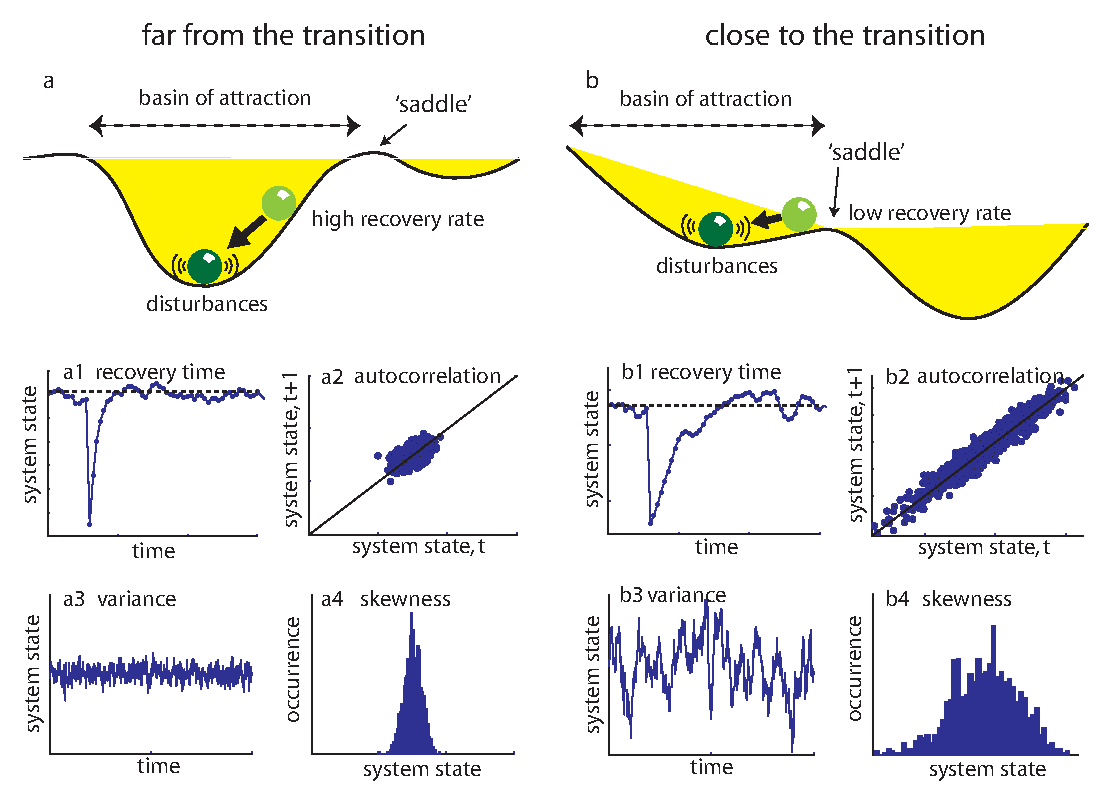
\includegraphics[scale=0.8]{figure1.eps}
\caption{Early-warnings in the dynamics of a system as it approaches a critical transition. Far from the transition resilience is high (a): the system lies in a broad and steep basin of attraction. Small disturbances are damped by high recovery rates back to equilibrium. As a result the time to recover from perturbations is short (a1), the dynamics are characterized by low correlation between subsequent states (a2), low variance (a3), and low skewness (a4). Close to transition resilience is low (b): the system lies in a narrow and flat basin of attraction. Small disturbances are not effectively damped due to critical slowing down. As a result the time to recover from perturbations is short (b1), the dynamics are characterized by high correlation (b2), high variance (b3), and high skewness (b4).}
\end{center}
\label{fig:ews_theory}
\end{figure}

\subsection{What are Early Warning Signals?}
While an increase in recovery time after a disturbance is the most direct indicator of the proximity to a tipping point, for most natural systems it will be very difficult to measure. Take for instance the impossibility of conducting a perturbation experiment for measuring recovery time of the thermohaline circulation in the Atlantic Ocean. There is, however, an alternative window of opportunity. As all systems are permanently subjected to natural perturbations, we may perhaps use these continuous disturbances to indirectly probe critical slowing down prior to a tipping point. Indeed, critical slowing down leads to an \textit{\textbf{increase in autocorrelation}} \cite{Ives1995,Held2004}: the state of the system today looks more like its state yesterday when it is close to a tipping point (Fig. 1a2, b2). %The resulting increase in `memory' of the system can be measured in the frequency spectrum of the system by simply looking at lag-1 autocorrelation in the pattern of fluctuations (Held \& Kleinen 2004). 
It also causes an \textit{\textbf{increase in variance}} \cite{Carpenter2006a}: as perturbations accumulate and are not damped sufficiently fast, the state of the system fluctuates more widely around its present state (Fig. 1a3, b3). In addition, the basin of attraction may become asymmetric close to a transition \cite{Scheffer2009a} (Fig. 1a, b). Such asymmetry may cause the state of the system to spend more time in the flatter part of the basin that leads to an \textit{\textbf{increase in skewness}} \cite{Guttal2008} in the distribution of the monitored system state before a transition (Fig. 1a4, b4).

\section{The Early Warning Signals Toolbox - Application}
\subsection{General characteristics}
The Early Warning Signals Toolbox is designed to \textbf{estimate} and \textbf{visualize} a series of \textbf{14 indicators} that reflect the effects of critical slowing down in a system approaching a critical transition (Table 1) \cite{Dakos2012a}. In particular, the toolbox:
\begin{itemize}
\item operates on time series collected by monitoring the state of a system that might undergo a critical transition. No other information than a time series is required. 
\item is generic and applicable to a wide variety of data sources, including temperature data, nutrient concentrations, microbial biomass, brain activity, stock marker indices or similar.
\item is applicable to both real world observations as well as simulations derived from models that are, for instance, developed to understand future scenarios, like climatic transitions, ecological shifts or social collapses.
\item It can be run locally from github over a network, or on a dedicated server and everything is always fully transparent. this has advantages over standard local executables that are more difficult to modify to new purposes, or non-transparent applications that can only be accessed through an external server interface
\end{itemize}


\begin{table}[h]
\centering
\caption{Indicators provided by the Early Warning Signals Toolbox}%\\[1ex]
\begin{tabular}{l l}% c c }
\hline
\hline
%\textbf{Indicator}\\%	&	Rising memory	&	Rising variability	&	Flickering	\\ [0.5ex]
%\hline
Autocorrelation at-lag-1 &	%&	x	&		&	\\
Autoregressive coefficient of AR(1) model	\\ %&	x	&		& 	\\
Return rate &	%&	x	&		&	\\
Spectral density \\%	&	x	&		&	\\
Spectral ratio &	%&	x	&		&	\\
Spectral exponent\\	%&	x	&		&	\\
Standard deviation &	%&		&	x	&	x	\\
Coefficient of variation\\	%&		&	x	&	x \\
Skewness &	%&		&	x	&	x \\
Kurtosis	\\%&		&	x	&	x \\
Conditional heteroskedasticity	&%&		&	x	&	x	\\
BDS test	\\%&		&	x	&	x	\\
Nonparametric drift-diffusion-jump models	&%&	x	&	x	&	x	\\
Potential analysis	\\ [0.5ex]%&		&		&	x	\\ [1ex]
\hline
\hline
\end{tabular}
\label{methods_table}
\end{table}%

\subsection{Using the toolbox - An example of tipping to overexploitation}
Consider a managing institution of a harvested resource (be it grazing grounds, or fish stocks) that has been monitoring a resource and is concerned with the risk of a regime shift due to increased harvesting pressure. The manager has been collecting a time series of the resource and is aware of a slight decline in resource biomass (Fig. 2), but it is difficult to assess the risk of reaching the point of no return at which the resource may tip to overexploitation. Thus, the manager is hesitant to restrict harvesting and start implementing a restoration program. 

\begin{figure}[h]
\begin{center}
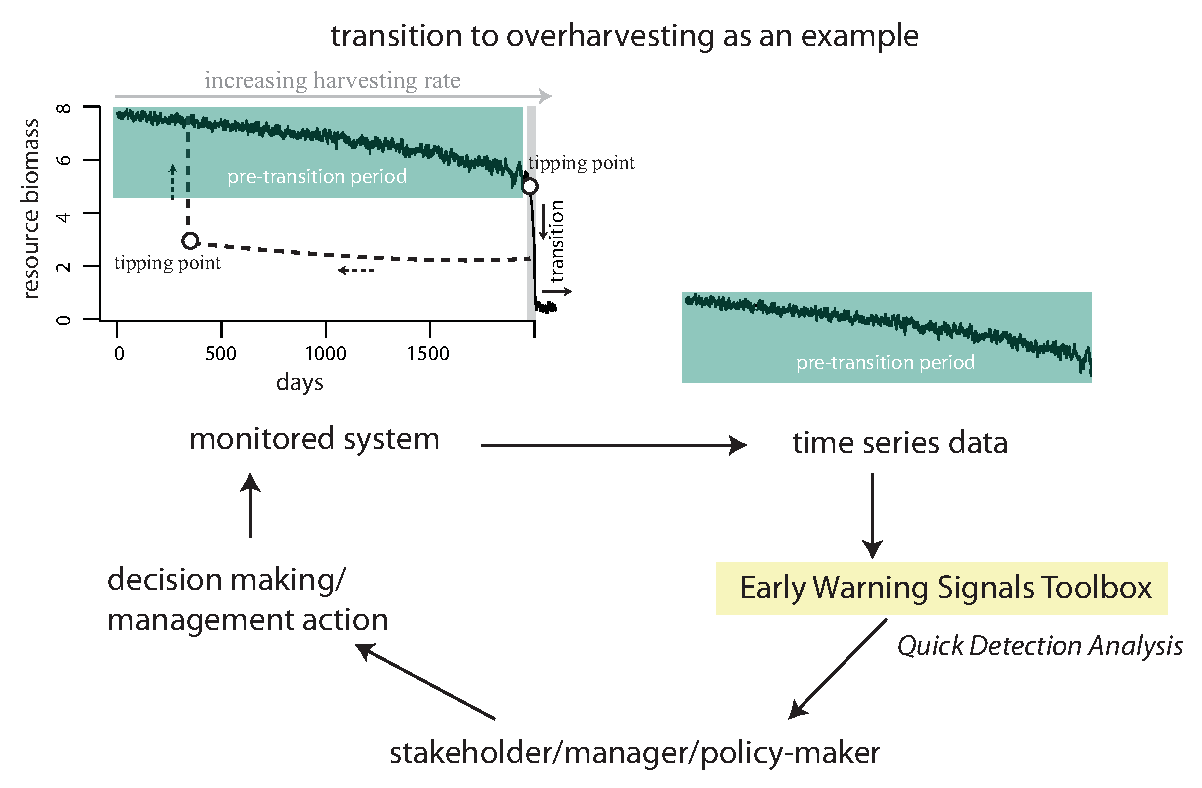
\includegraphics[scale=0.75]{figure_workflow.eps}
\caption{Simulated data of a collapsing overharvested resource as an example of how the Early Warning Signals Toolbox can inform decision making on the management of complex systems. It is supposed that there is access only to the pre-transition data.}
\end{center}
\label{fig:data}
\end{figure}

However, the manager has now at her disposal the \textbf{\textit{Early Warning Signal Toolbox}}. The toolbox allows her to regularly run a \textbf{\textit{Quick Detection Analysis (QDA)}} online on a personal computer to quantify the resilience of the system and the risk of approaching a tipping point. In this case, the manager finds out that after removing the slow declining trend in mean resource biomass (red line in Fig. 3a), the residuals (Fig. 3b) show a rise in autocorrelation and variance when estimated within sliding windows along the monitored time series (Fig. 3c, d). %Sensitivity analysis to the parameters of the time series analysis do not change the result: different parameter choices give positive trends in autocorrelation and variance (Fig. 2B). The system indeed seems to be close to tipping, as the resilience is low. 
Interestingly, the estimated positive trends in the two indicators (0.914 for autocorrelation and 0.699 for variance) are alarming signals for a decline in the system's resilience and a potential tipping.

But how significant are these trends? From the drop-down menu of the \textbf{QDA} (box 1), the manager performs a trend significance analysis to test if the same trends estimated from the monitored data could also be found by chance. The significance analysis (Fig. 4) shows that the trend in autocorrelation is significant at a level below 0.05, and the trend in variance is close to being significant at the same level. The manager now is starting to have serious concerns that the resource is losing resilience and tipping may not be that far. 

Could it be that the resource has also passed the point of no return and started moving to the overharvested alternative state? \textbf{QDA} offers the possibility to explore whether an alternative attractor has already appeared by performing a potential analysis. In this case, however, potential analysis does not support such conclusion (Fig. 5). Still the resource is riding the current underexploited state. Perhaps there is still time to take action and avoid further undermining the resilience of the resource!\\

%\begin{figure}[ht]
%\begin{center}
%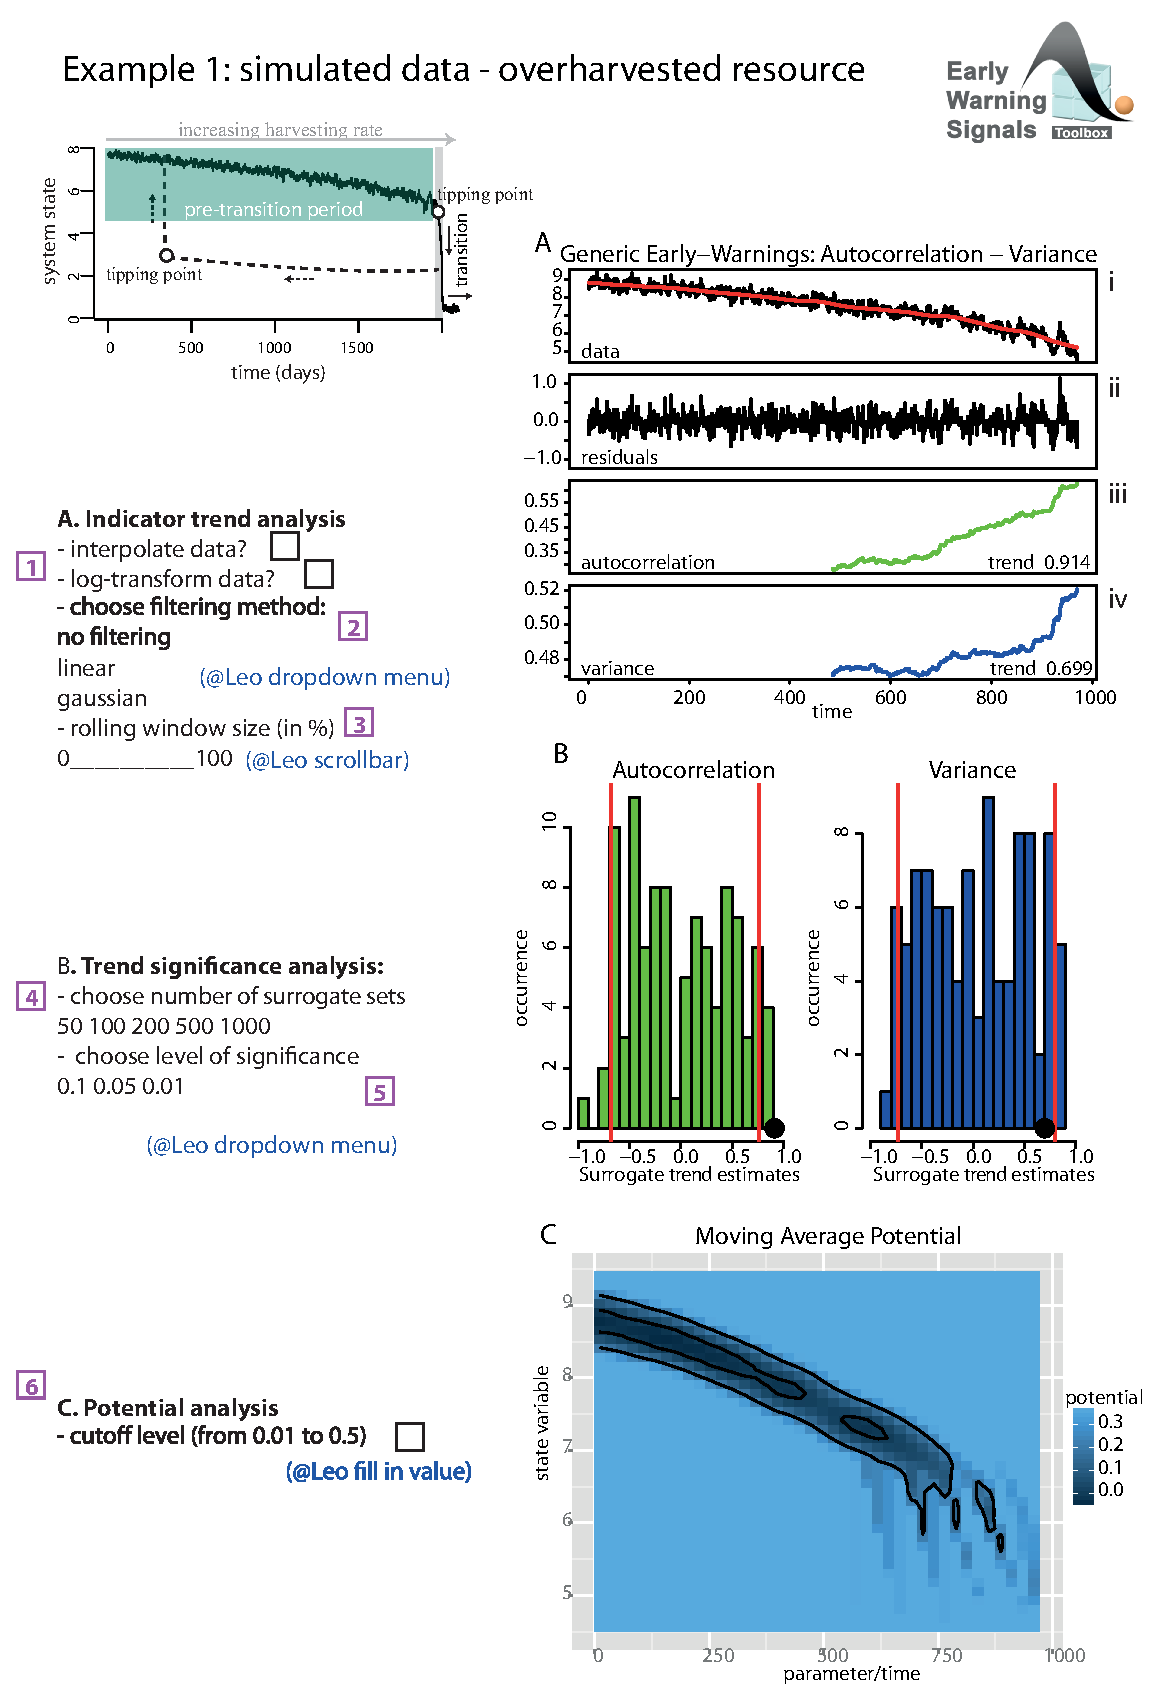
\includegraphics[scale=0.6]{fig_2_simulated_970pts.eps}
%\caption{Demo Quick Detection Analysis in simulated data prior to shifting to overexploitation}
%\end{center}
%\label{fig:simulatedQDA}
%\end{figure}

The above \textbf{Quick Detection Analysis} estimates the flagship indicators for the detection of critical transitions and is only part of the full functionality of the toolbox (see \ref{sec:resources}). QDA works in an interactive environment that allows the user to directly perform the analysis with a time series as solely input.
In detail, \textbf{QDA} performs three operations:
\begin{enumerate}
\item \textbf{Indicator trend analysis} of autocorrelation and variance along a time series based on sliding windows. The user can optionally log-transform or interpolate data (eg. if there are missing values or the data are unevenly spaced) (Fig. 3, box 4), as well as filter the data using smooth, linear, or first-difference detrending from a drop-down menu (Fig. 3, box 3). It is also possible to select the size of the sliding window (defined as a fraction of the time series length) (Fig. 3, box 2).
\item \textbf{Trend significant analysis} of autocorrelation and variance. Two drop-down menus allow the user to choose the number of surrogate datasets and the level of significance to control the  (Fig. 4, box 1, 2). 
\item \textbf{Potential analysis} for reconstructing the potential landscape of the system states, which helps to identify alternative attractors from the data. The user can choose the threshold for the detection of alternative attractors (Fig. 5, box 1), the number of points to evaluate the potential (Fig. 5, box 2), as well as a cutoff level for the visualization of the alternative attractors (Fig. 5, box 3).
\end{enumerate}

Interested to know how \textbf{QDA} works for a real-world example? Select \textit{real climate data} from the drop-down menu (as shown in Fig. 3 box 1), and try to detect yourself the Earth's last climate shift from a cold period to the stable climate conditions as we know them today!

%\begin{figure}[h]
%\begin{center}
%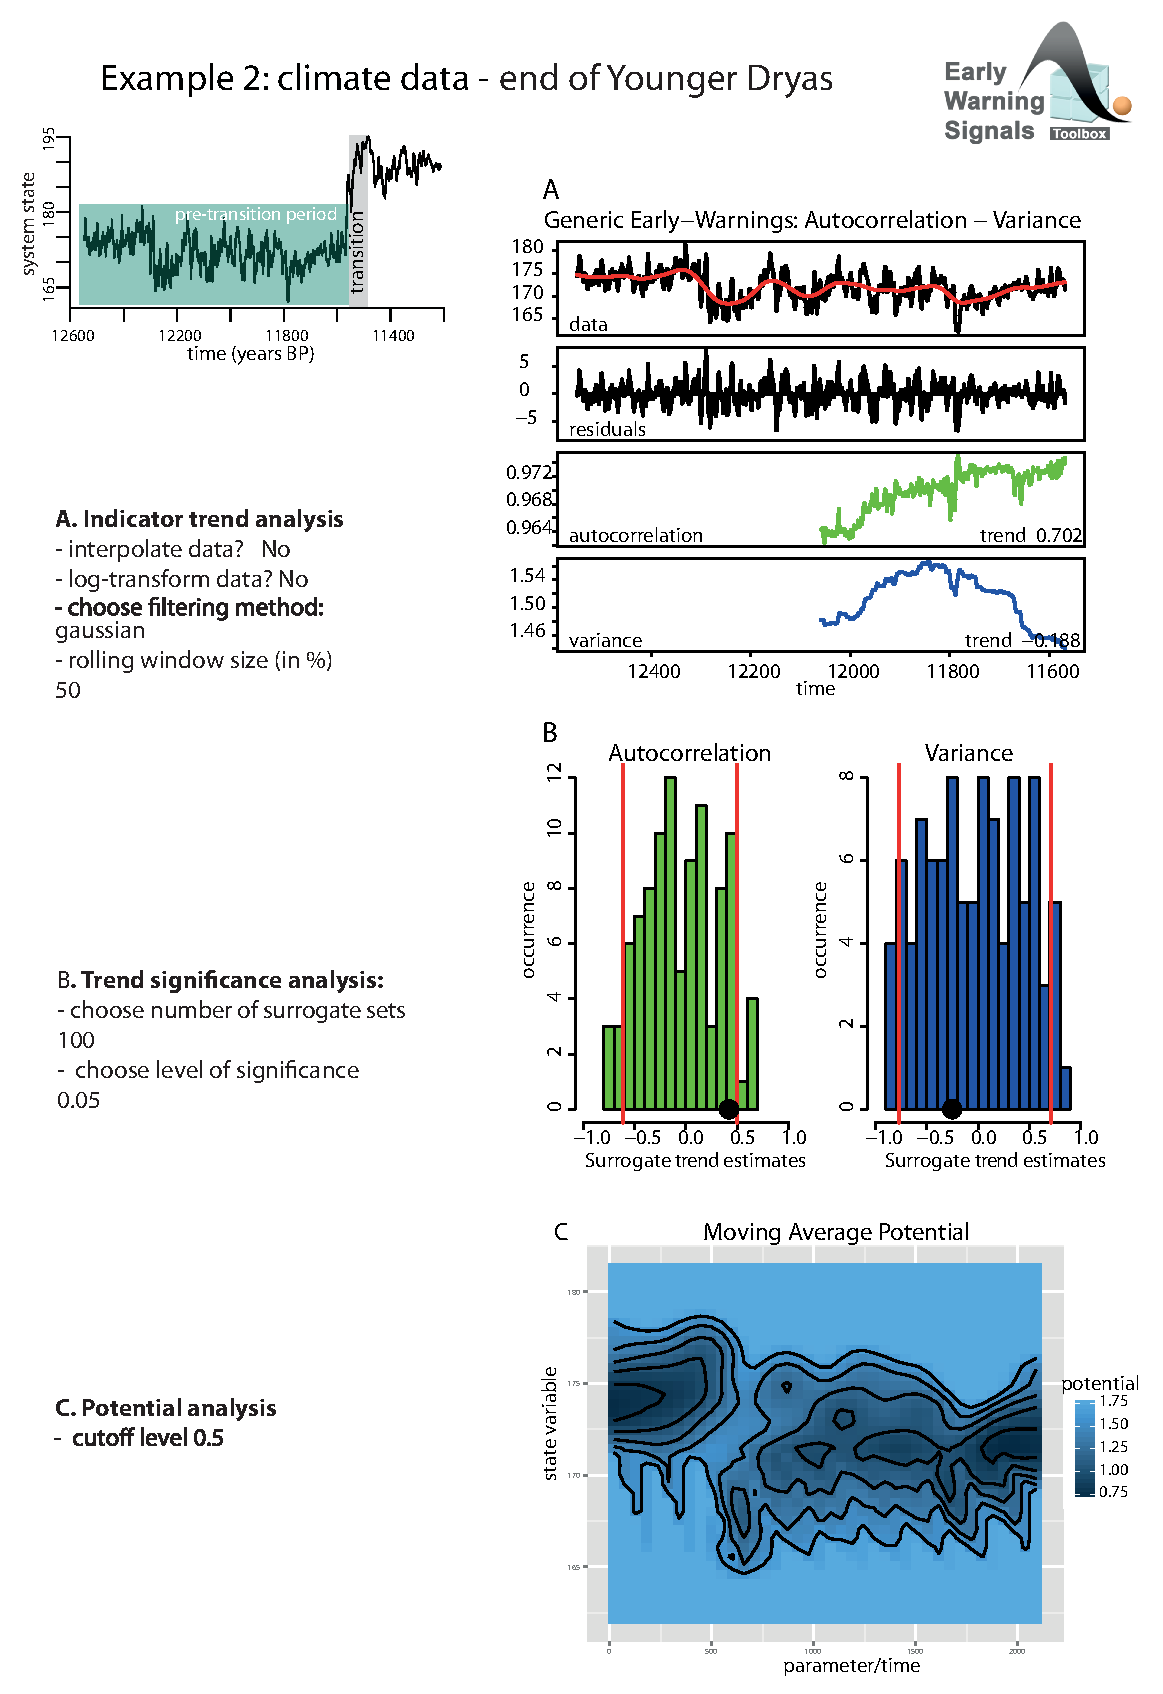
\includegraphics[scale=0.8]{fig_3_climatedata.eps}
%\caption{Quick Detection Analysis for the climate records prior to the exit from the Younger Dryas around 11,500 ago.}
%\end{center}
%\label{fig:QDA_climate}
%\end{figure}

\subsection{Resources} 

\label{sec:resources}
Our innovative contribution does not stop only at the toolbox. We have made available a complete set of resources to understand the methodology, apply the tools, and encourage its further development. In particular:
\begin{itemize}
\item The toolbox is supported by a dedicated \textbf{Early Warning Signals website}\footnote{\url{http://www.early-warning-signals.org}} that hosts all theoretical and practical background information, original publications, case studies, and updates of the science around the theme of early warnings and critical transitions. 
\item The toolbox is developed and hosted in the widely-used open-source statistical language \textbf{\textit{R}}, which means that it is ready-to-use, constantly maintained, and fully documented\footnote{\url{http://cran.r-project.org/web/packages/earlywarnings/index.html}}\footnote{\url{https://github.com/earlywarningtoolbox/earlywarnings-R/blob/master/earlywarnings-manual.pdf}}.
 \item Our project development version is available under an open source license to download on any operating system from \textbf{github}\footnote{\url{https://github.com/earlywarningtoolbox}}: an open-access, free-sharing platform that makes the further development of our toolbox transparent and incredibly easy.
 \end{itemize}

%\href{http://www.early-warning-signals.org}{webpage}
%\href{http://cran.r-project.org/web/packages/earlywarnings/index.html}{CRAN repository}, 
%\href{https://github.com/earlywarningtoolbox}{github}

\section{Potential impact and future perspectives}
The \textbf{Early Warning Signals Toolbox} presents a state-of-the-art approach for detecting generic indicators of critical transitions in time series for a wide range of systems. Derived from a solid theoretical background and given the increasing availability of time series monitoring data (e.g. from tweeter, remote sensing, to high throughput data), the toolbox can provide a new perspective for anticipating and managing transitions in cases as diverse as fisheries, ocean circulation patterns, migraine attacks, psychological disorders, or social transformations. It is flexible, easy-to-use, and designed with a community-based computing philosophy. Additionally, its interactive user-friendly character increases its potential for becoming a fast diagnostic test for scientists, managers, as well as policy-makers. For this proposal, we have demonstrated only part of the capacities of our toolbox. Our aim is to develop the complete content of the Early Warning Signals Toolbox into an interactive, ready-to-use interface. We hope that the WICC Data Challenge will offer us this opportunity.\\

\end{doublespacing}
\newpage
{\small
\textbf{Acknowledgements}
We are grateful to Steve Carpenter, Buz Brock, Aaron Ellison, Vishwesha Guttal, Tony Ives, Sonia K\'{e}fi, Valerie Livina, David Seekell, Tim Cline, Egbert van Nes, and Marten Scheffer for sharing and developing their work that is inherent part of the Early Warning Signals Toolbox. Also we thank the Synergy Program for Analyzing Resilience and Critical Transitions  (SPARCS) for supporting our initiative.

 %
\bibliographystyle{unsrt}
 %
\bibliography{WICC_bibl}
 %
}

\newpage
\begin{figure}[ht]
\begin{center}
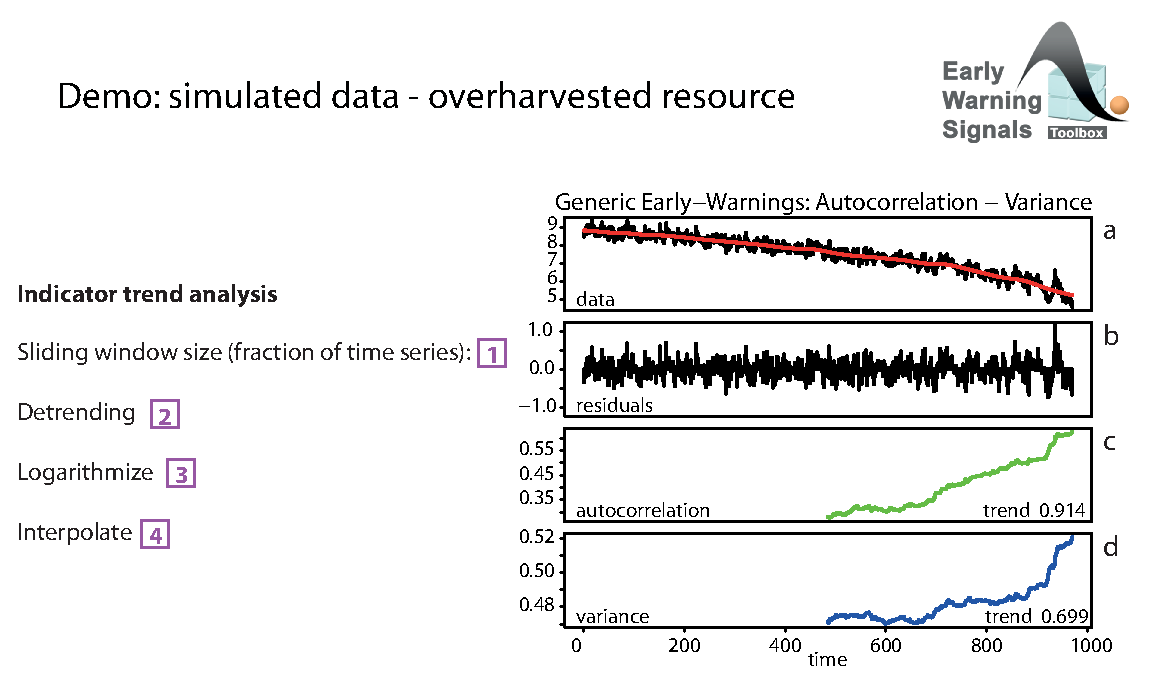
\includegraphics[scale=0.8]{fig_3_simulated_generic.eps}
\caption{Demo Quick Detection Analysis: \textbf{Indicator trend analysis} in simulated data prior to shifting to overexploitation.}
\end{center}
\label{fig:simulated_generic}
\end{figure} 

\newpage
\begin{figure}[ht]
\begin{center}
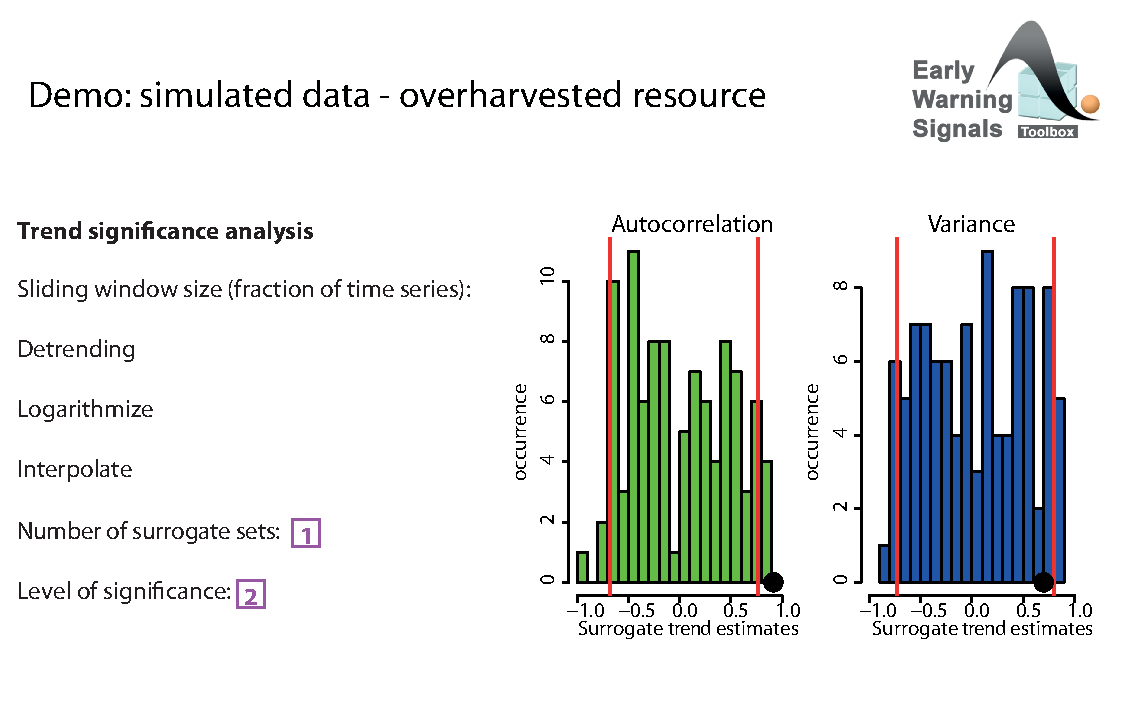
\includegraphics[scale=0.8]{fig_4_simulated_significance.eps}
\caption{Demo Quick Detection Analysis: \textbf{Trend significance analysis} in simulated data prior to shifting to overexploitation.}
\end{center}
\label{fig:simulated_significance}
\end{figure} 

\newpage
\begin{figure}[ht]
\begin{center}
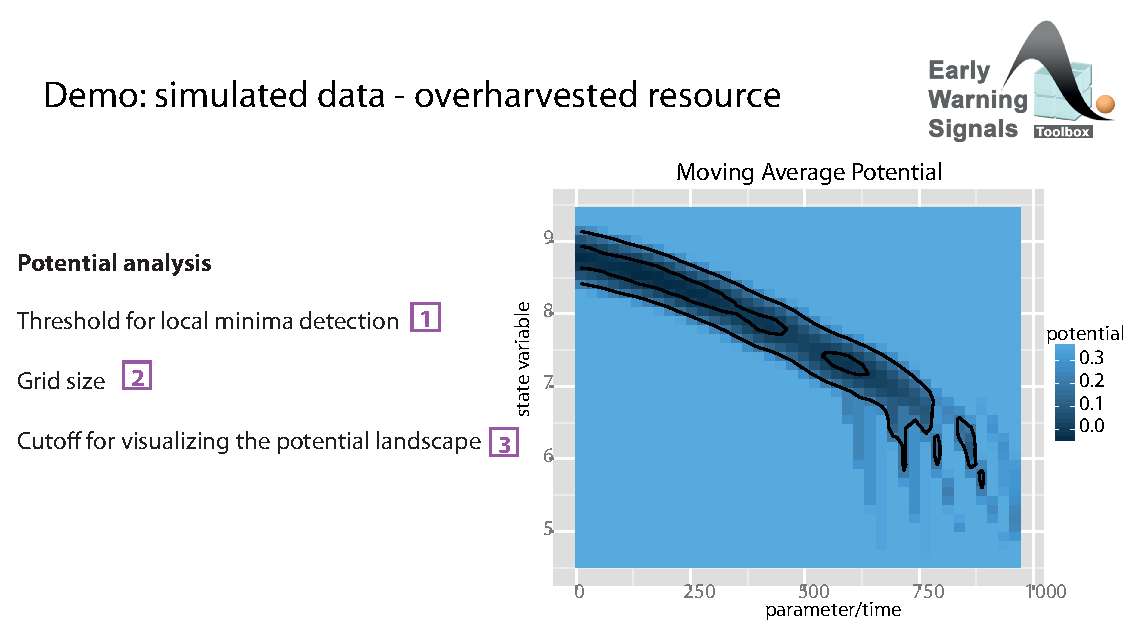
\includegraphics[scale=0.8]{fig_5_simulated_potential.eps}
\caption{Demo Quick Detection Analysis: \textbf{Potential analysis} in simulated data prior to shifting to overexploitation.}
\end{center}
\label{fig:simulated_potential}
\end{figure} 

\end{document}

